\documentclass{beamer}


% Load essential packages
\usepackage{hyperref} % Only load once to avoid conflicts
\usepackage{stile}
\usepackage{subcaption}
\usepackage{tcolorbox}
\usepackage[font=scriptsize,skip=1pt]{caption}
\usepackage[T1]{fontenc}
\usepackage{csquotes}
\usepackage[backend=biber, style=authoryear, maxnames=3, minnames=1, abbreviate=false, date=long, url=false, isbn=false, doi=false]{biblatex}
\addbibresource{lecture9/bib.bib} % Ensure this matches your bibliography file name

\interfootnotelinepenalty=10000

\usepackage{latexsym, amsmath, xcolor, multicol, booktabs, calligra}
\usepackage{graphicx, pstricks, listings, stackengine}

% Hyperref setup
\hypersetup{
    hidelinks,
    colorlinks=true,
    linkcolor=black,
    citecolor=blue,
    urlcolor=black
}

% Font theme for Beamer
\usefonttheme[onlymath]{serif}

% Custom definitions
\def\cmd#1{\texttt{\color{red}\footnotesize $\backslash$#1}}
\def\env#1{\texttt{\color{blue}\footnotesize #1}}
\definecolor{deepblue}{rgb}{0,0,0.5}
\definecolor{deepred}{rgb}{0.6,0,0}
\definecolor{deepgreen}{rgb}{0,0.5,0}
\definecolor{halfgray}{gray}{0.55}

% Beamer color settings
\setbeamercolor{block title}{bg=blue!70!white, fg=white}
\setbeamercolor{block body}{bg=blue!10!halfgray, fg=white}
\setbeamercolor{section in head/foot}{fg=white}
\setbeamercolor{subsection in head/foot}{fg=white}
\setbeamercolor{title in head/foot}{fg=white}


% Listings settings for code highlighting
\lstset{
    basicstyle=\ttfamily\small,
    keywordstyle=\bfseries\color{deepblue},
    emphstyle=\ttfamily\color{deepred},
    stringstyle=\color{deepgreen},
    numbers=left,
    numberstyle=\small\color{halfgray},
    rulesepcolor=\color{red!20!green!20!blue!20},
    frame=shadowbox,
}

% Title page info
\author{Freya Rubel}
\title{Trade, Migration and Global Challenges}
\subtitle{Determinants of Migration}
\institute{}
\date{04.12.2025}

\graphicspath{{lecture9/}}

\begin{document}

\begin{frame}
    \titlepage
\end{frame}

\begin{frame}
    \tableofcontents[sectionstyle=show, subsectionstyle=show/shaded/hide, subsubsectionstyle=show/shaded/hide]
\end{frame}

\section{Introduction}
\begin{frame}{What is Migration?}
    \begin{itemize} \small
        \item Internal migration: movement of people from one area of a country to another.
        \item External migration: movement of people across national borders.
        \begin{itemize}
            \item To \textbf{emigrate} means to leave one's country of birth to live in another. 
            \item To \textbf{immigrate} means coming to another country that isn't your country of birth to live there.
        \end{itemize}
        \item Historical context: 
        \begin{itemize} \footnotesize
            \item Humans have for most of history lived a nomadic lifestyle and changed location as a result of food scarcity or climatic conditions.
            \item First settlements appeared around 10.000 years ago (with the beginning of the holocene).
        \end{itemize}
    \end{itemize}
\end{frame}

\begin{frame}{Overview - Migration in Modern History I}
    \textbf{18th century}
    \begin{itemize} \small
        \item European migration to the Americas.
        \item Forced migration of enslaved people ("transatlantic slave trade") mainly from Africa to the Americas.
        \item Industrialization encouraged increased urbanization.
    \end{itemize}
    \textbf{19th century}
    \begin{itemize} \small
        \item Peak of European migration to the Americas.
        \item Continued enslavement and displacement of people to European colonies and the Americas.
        \item Nationalism and Imperialism lead to forced displacement (e.g., the displacement of the Cherokee and other Native Americans to reservations).
    \end{itemize}
\end{frame}

\begin{frame}{Overview - Migration in Modern History II}
     \textbf{20th century}
    \begin{itemize} \small
    \item U.S.: large internal migration related to industrialization, racial discrimination, and environmental upheaval. % African Americans were subject to segregation in the south and the more industrialized cities in the north saw a shortage of workers and labor as the migration from Europe stopped due to the first world war
        \item The holocaust was preceded by migration waves fleeing persecution by the Nazis; millions of Germans and Poles had to move westward after European borders were redrawn.
        \item Upon the partition of India in 1947, large parts of the populations moved from India to Pakistan and vice versa.
    \end{itemize}
    \textbf{21st century}
    \begin{itemize} \small
        \item Beginning 2004, the EU granted EU citizens freedom of movement and residence within the EU.
        \item While European countries were mainly the source of immigration from the 15th century until the first half of the 20th century, the trend has reversed.
        \item Major Western cities see a rise in foreign students and professionals.
    \end{itemize}
\end{frame}

\begin{frame}{Trends in Foreign-Born Population}
    \begin{figure}
        \centering
        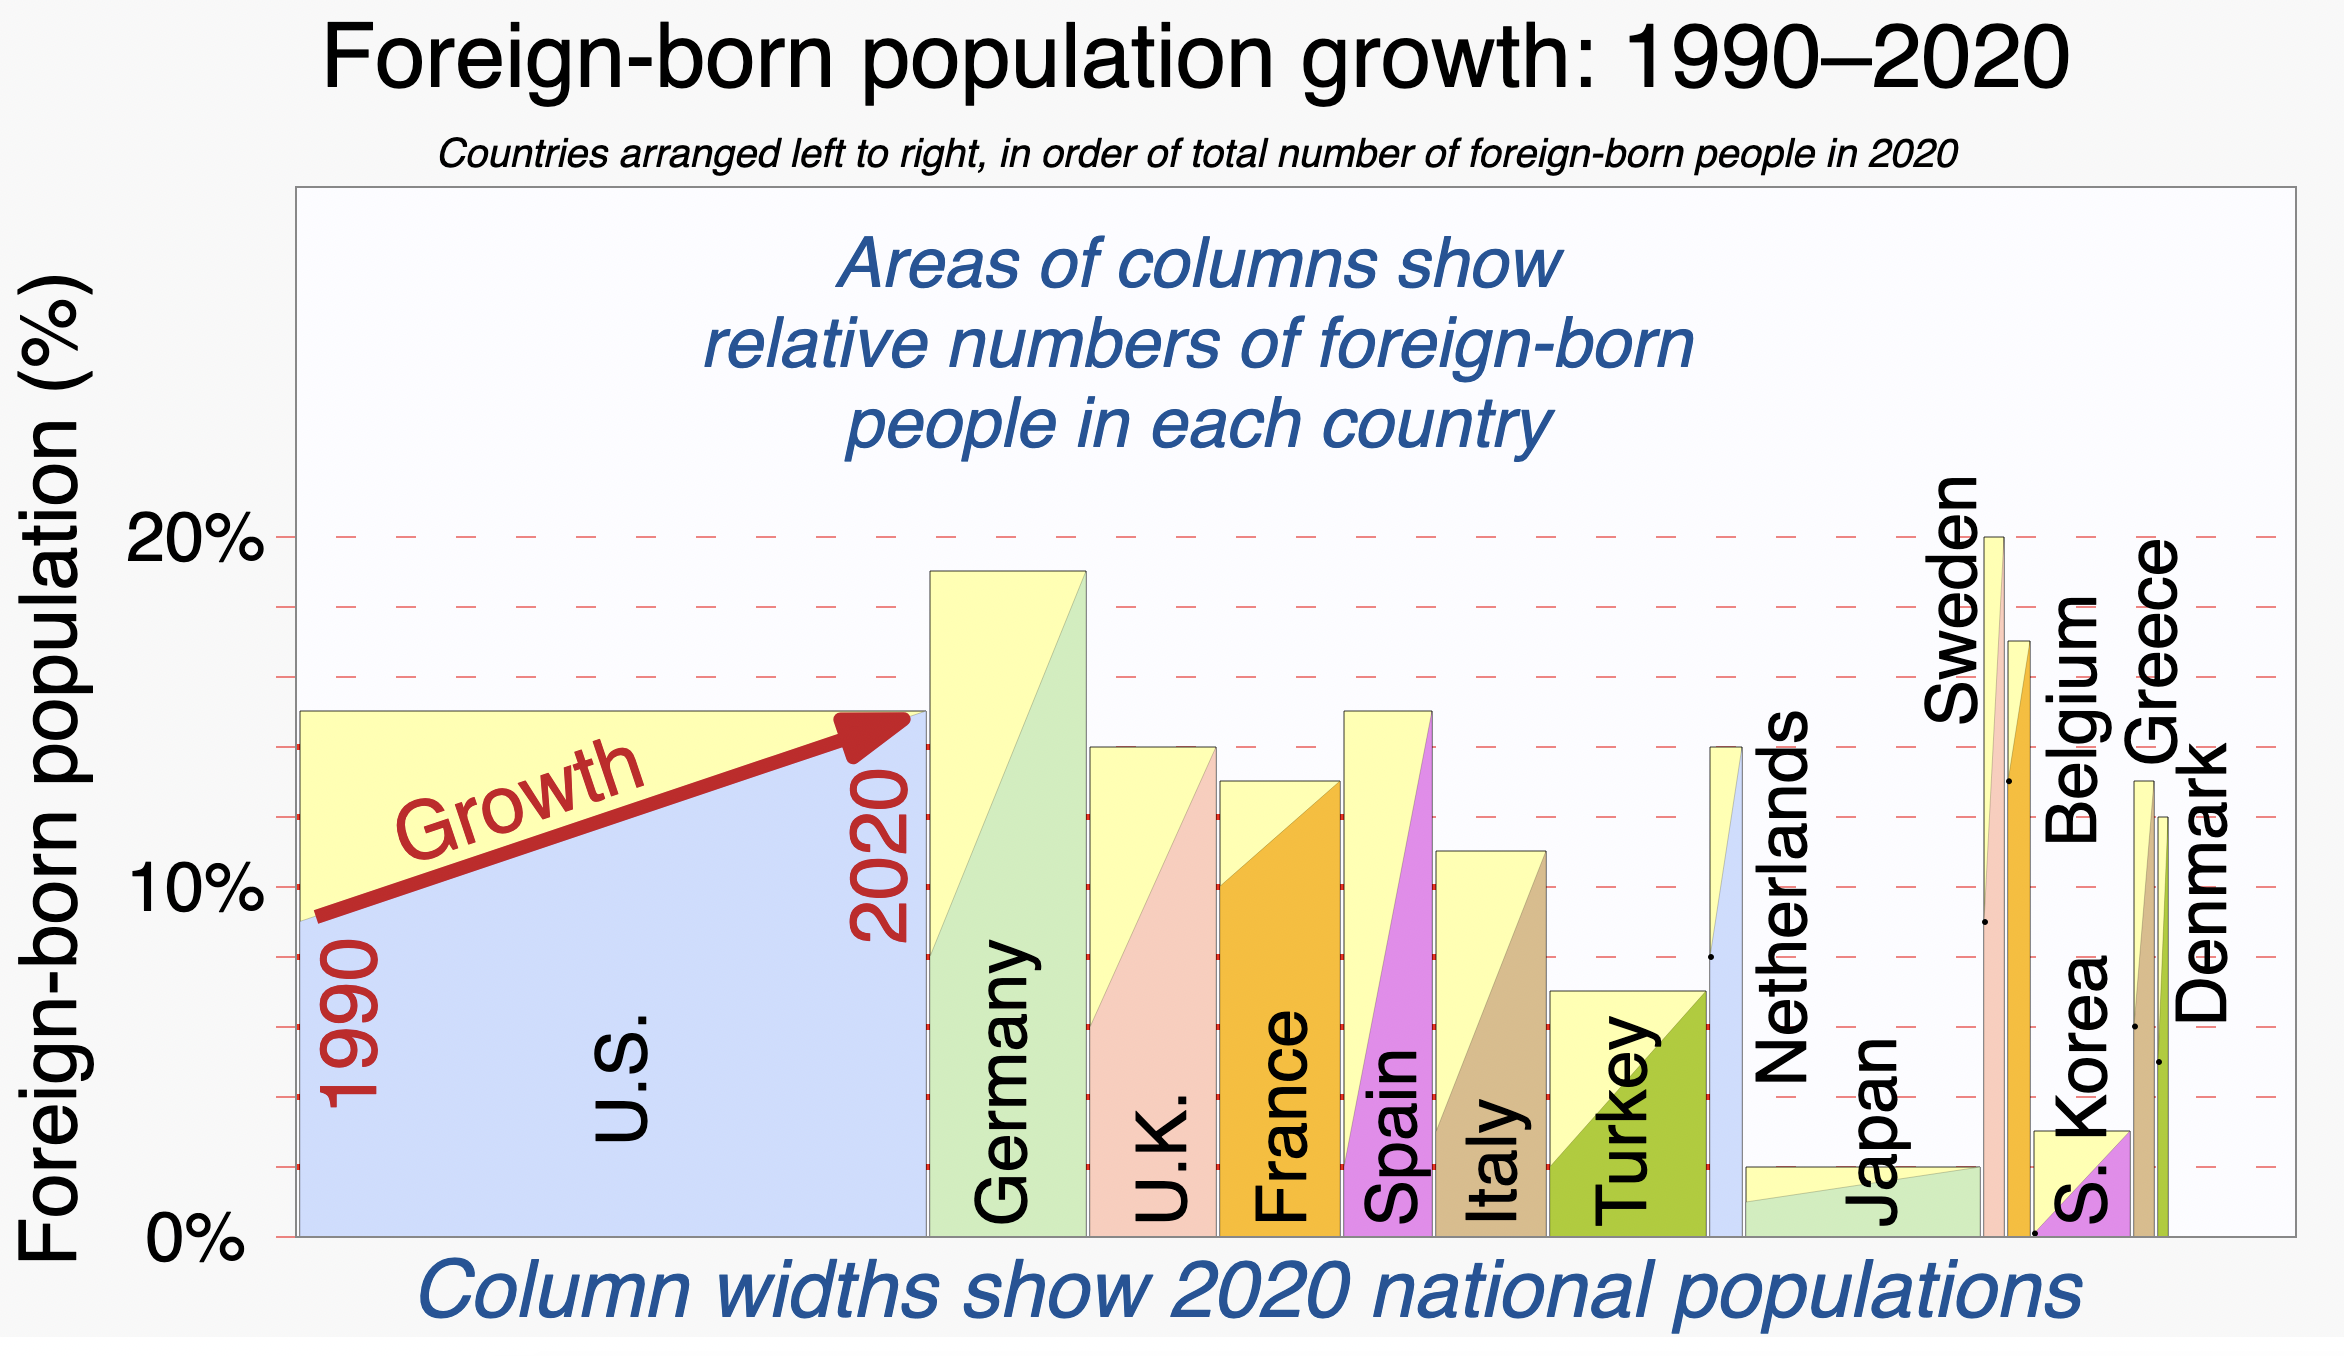
\includegraphics[width=\linewidth]{trend foreign born population.png}
        \label{fig:enter-label}
    \end{figure}
\end{frame}

\begin{frame}{Share of Foreign-Born Poeple (External Migrants)}
    \begin{figure}
        \centering
        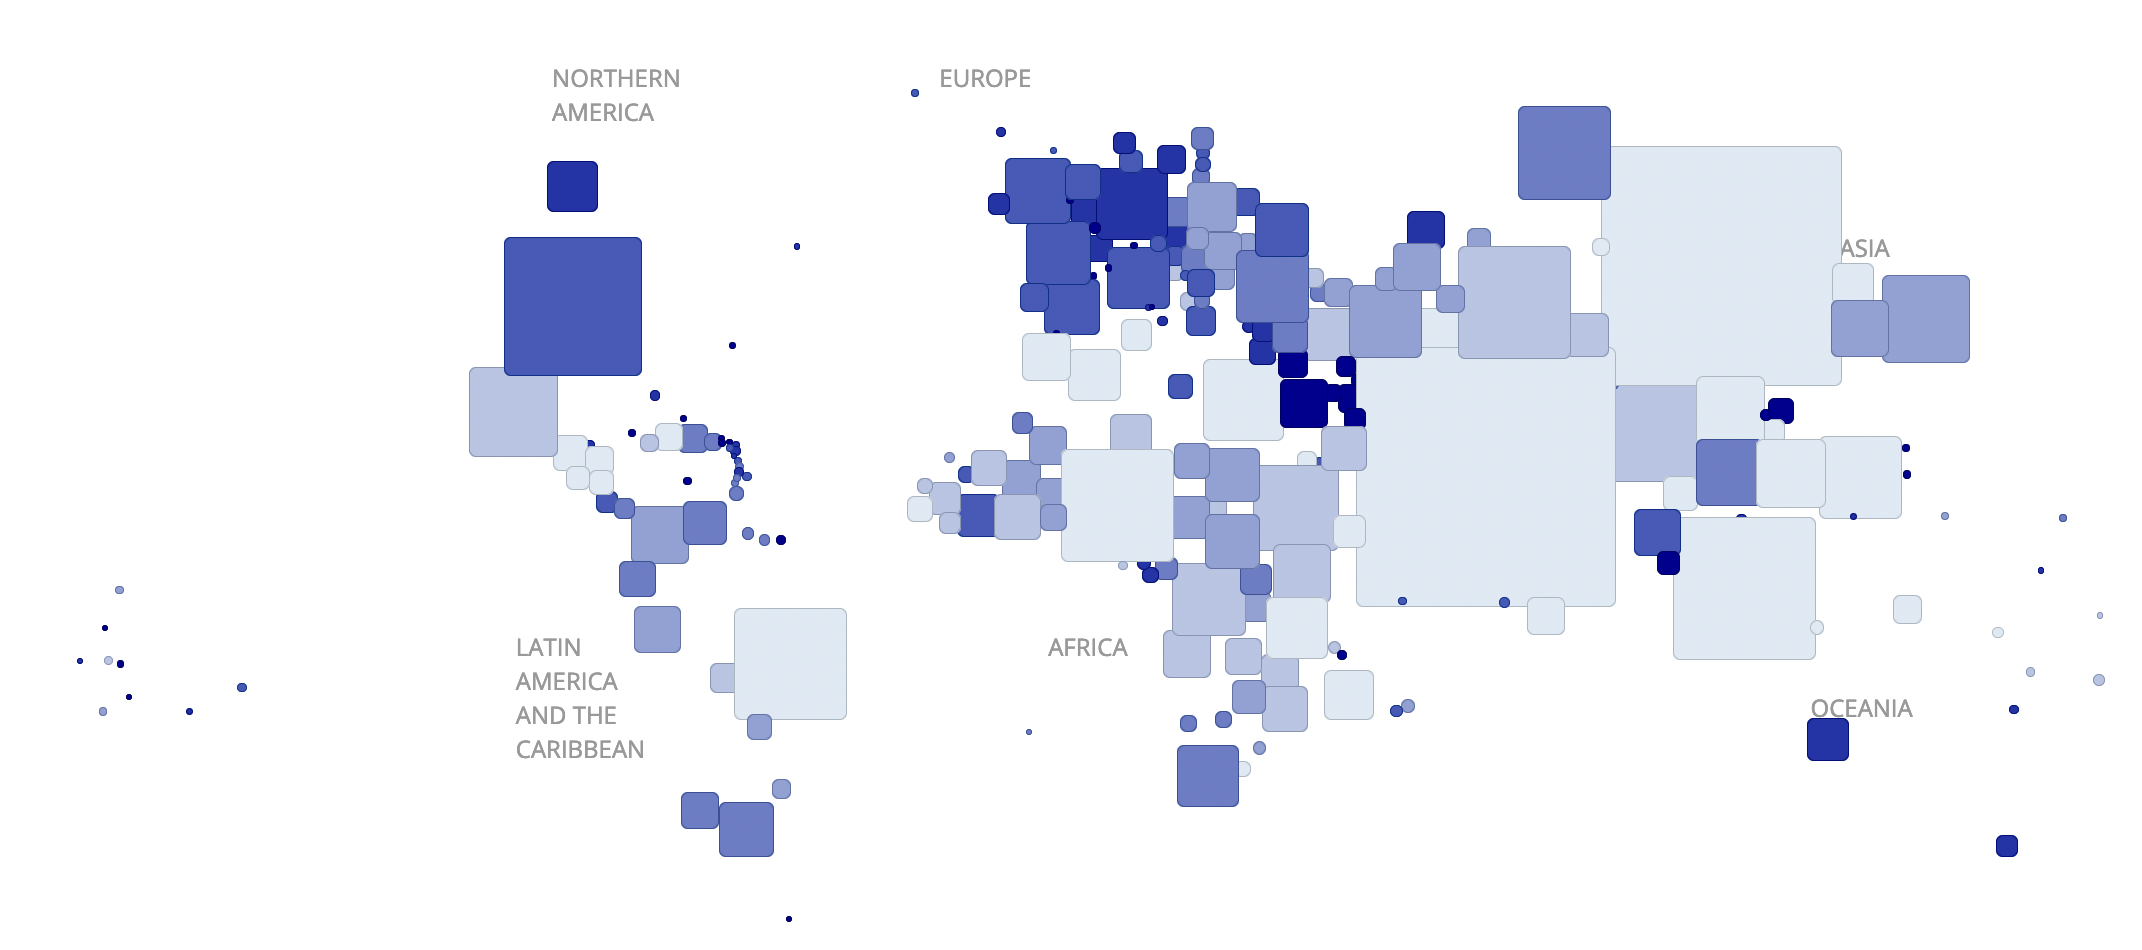
\includegraphics[width=\linewidth]{share international Migrants.png}
        \label{fig:enter-label}
    \end{figure}
\end{frame}

\begin{frame}{Why do Economists study Migration?}
    \begin{itemize} \small
        \item Migration does not only entail the movement of people, but also the movement of the factor ''labor''.
        \item Migration can stimulate technological advancements through a dissemination of knowledge and know-how.
        \item Migration has, especially in recent years, contributed to a rise in political tensions and thereby directly affected the political economy.
        \item Migration creates financial flows (remittance) that can impact economic development and poverty alleviation. 
    \end{itemize}
\end{frame}

\section{Economic Drivers}

\begin{frame}{Economic Opportunities}
    \textbf{Push Factors} \\
    \begin{itemize} \small
        \item Unemployment and low wages in the home country
        \item Poverty
        \item Economic inequality
        \item High costs of living
    \end{itemize}
    \textbf{Pull Factors}
    \begin{itemize} \small
        \item Economic stability
        \item Favorable business environment
        \item Demand for labor, higher wages, job opportunities
        \item Educational and training opportunities
    \end{itemize}
\end{frame}

\begin{frame}{Graphic Illustration I}
\begin{figure}
    \centering
    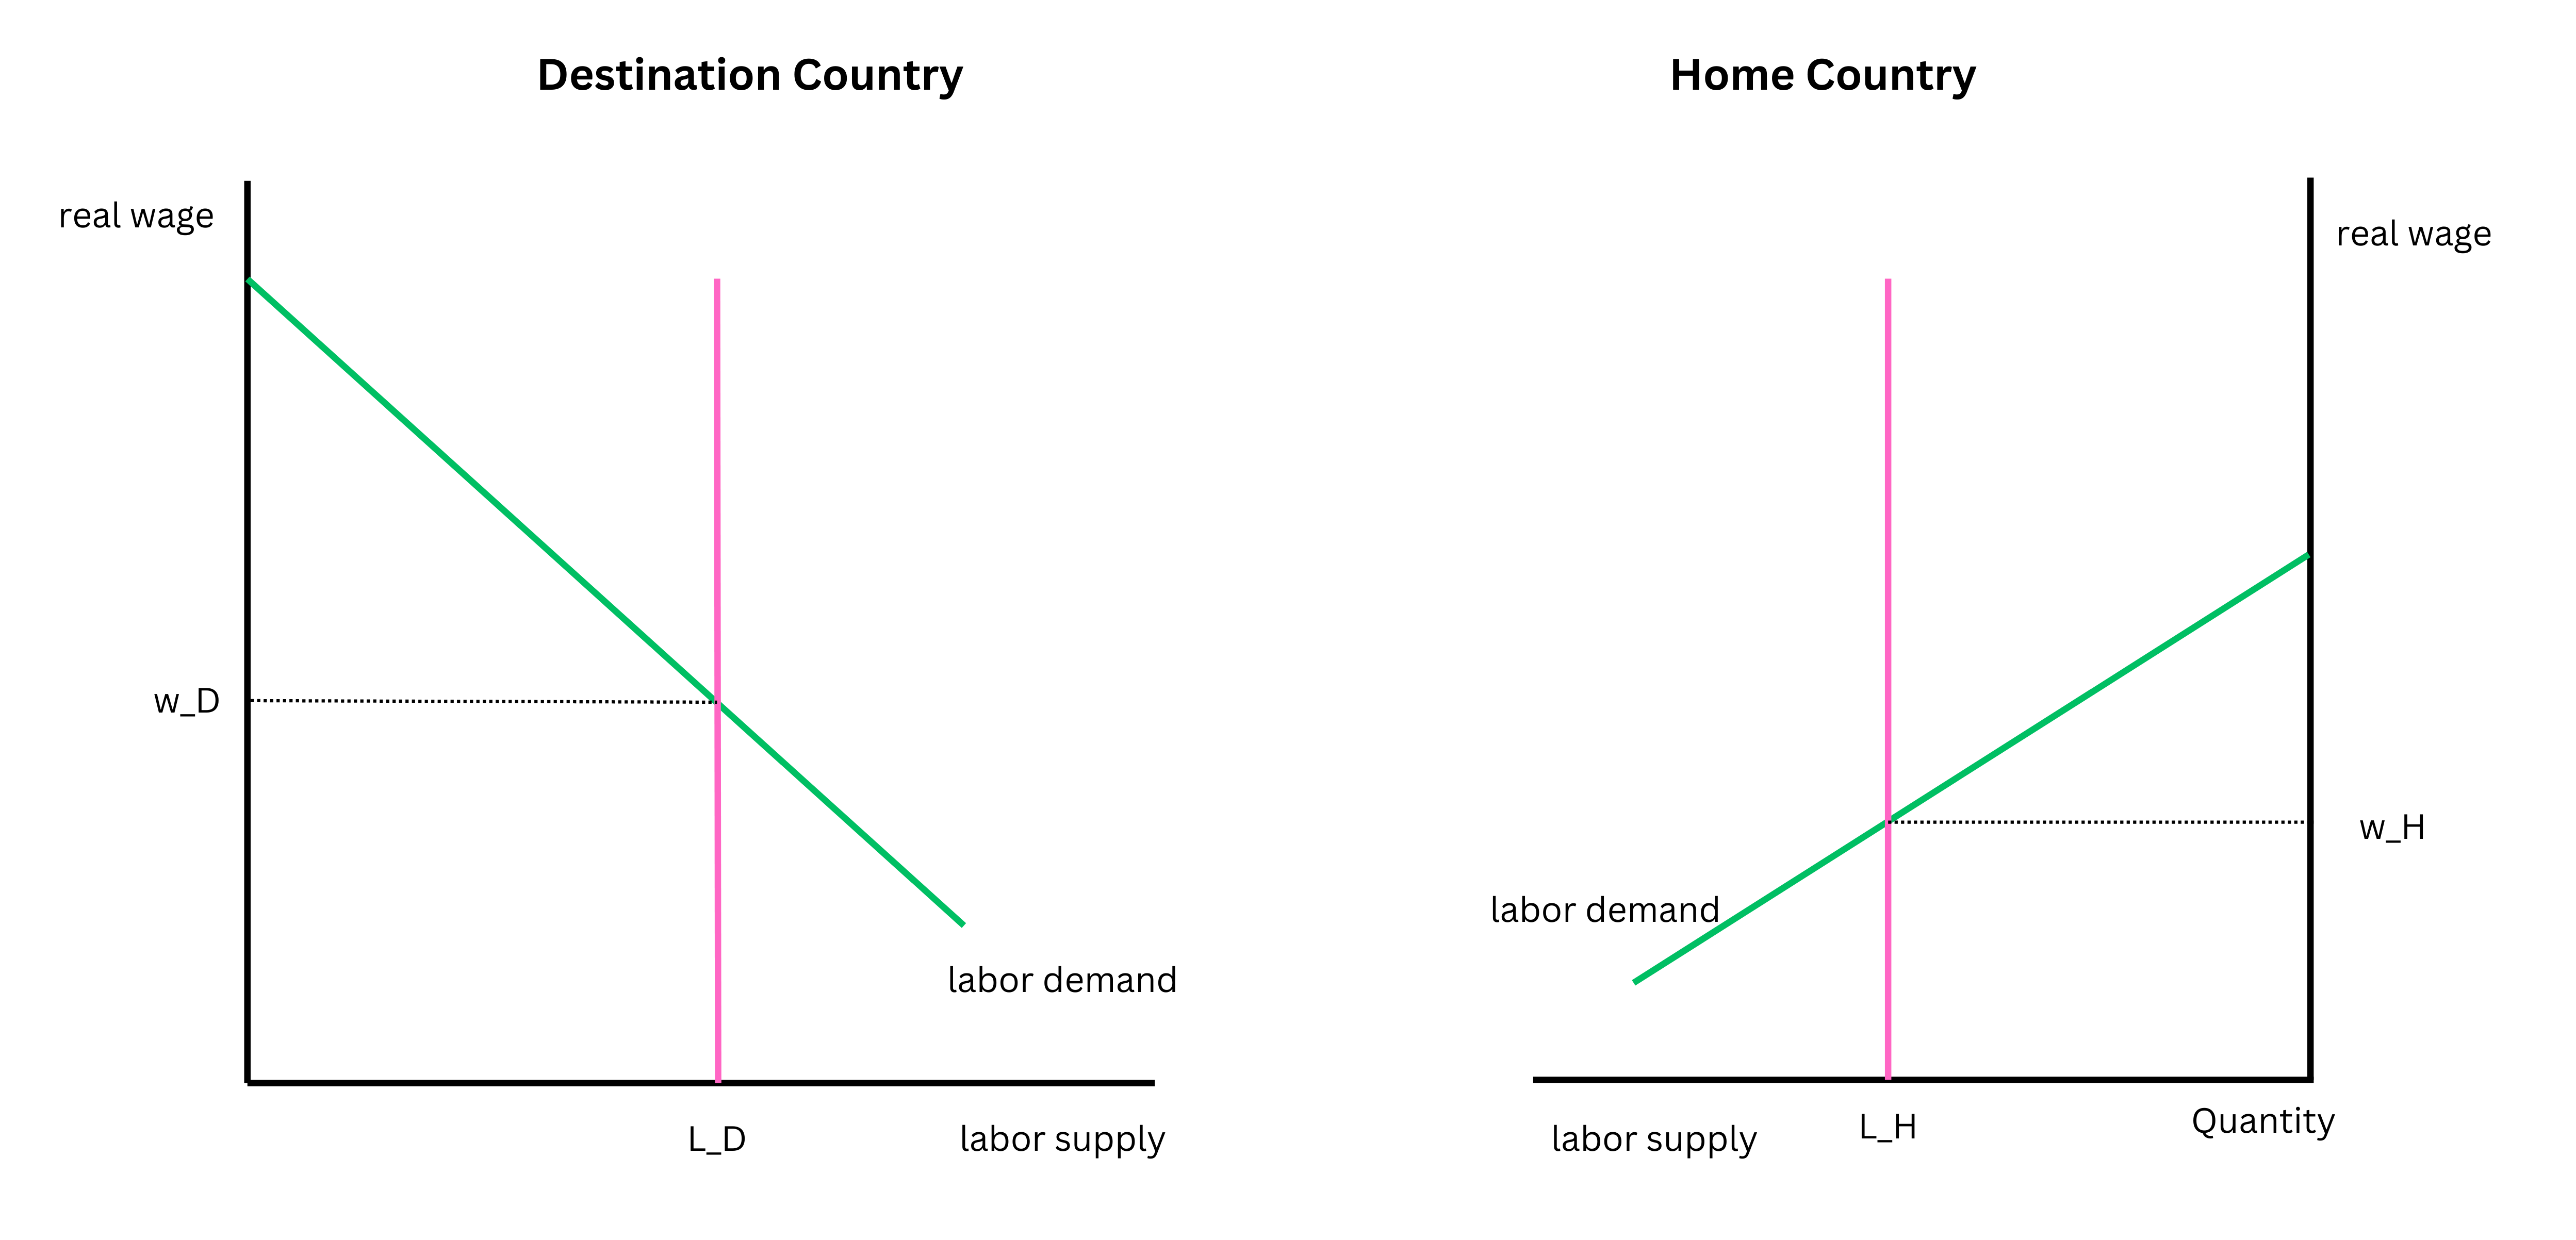
\includegraphics[width=\linewidth]{differences in wages.png}
    \label{fig:enter-label}
\end{figure} 
\end{frame}

\begin{frame}{Graphic Illustration II}
\begin{figure}
    \centering
    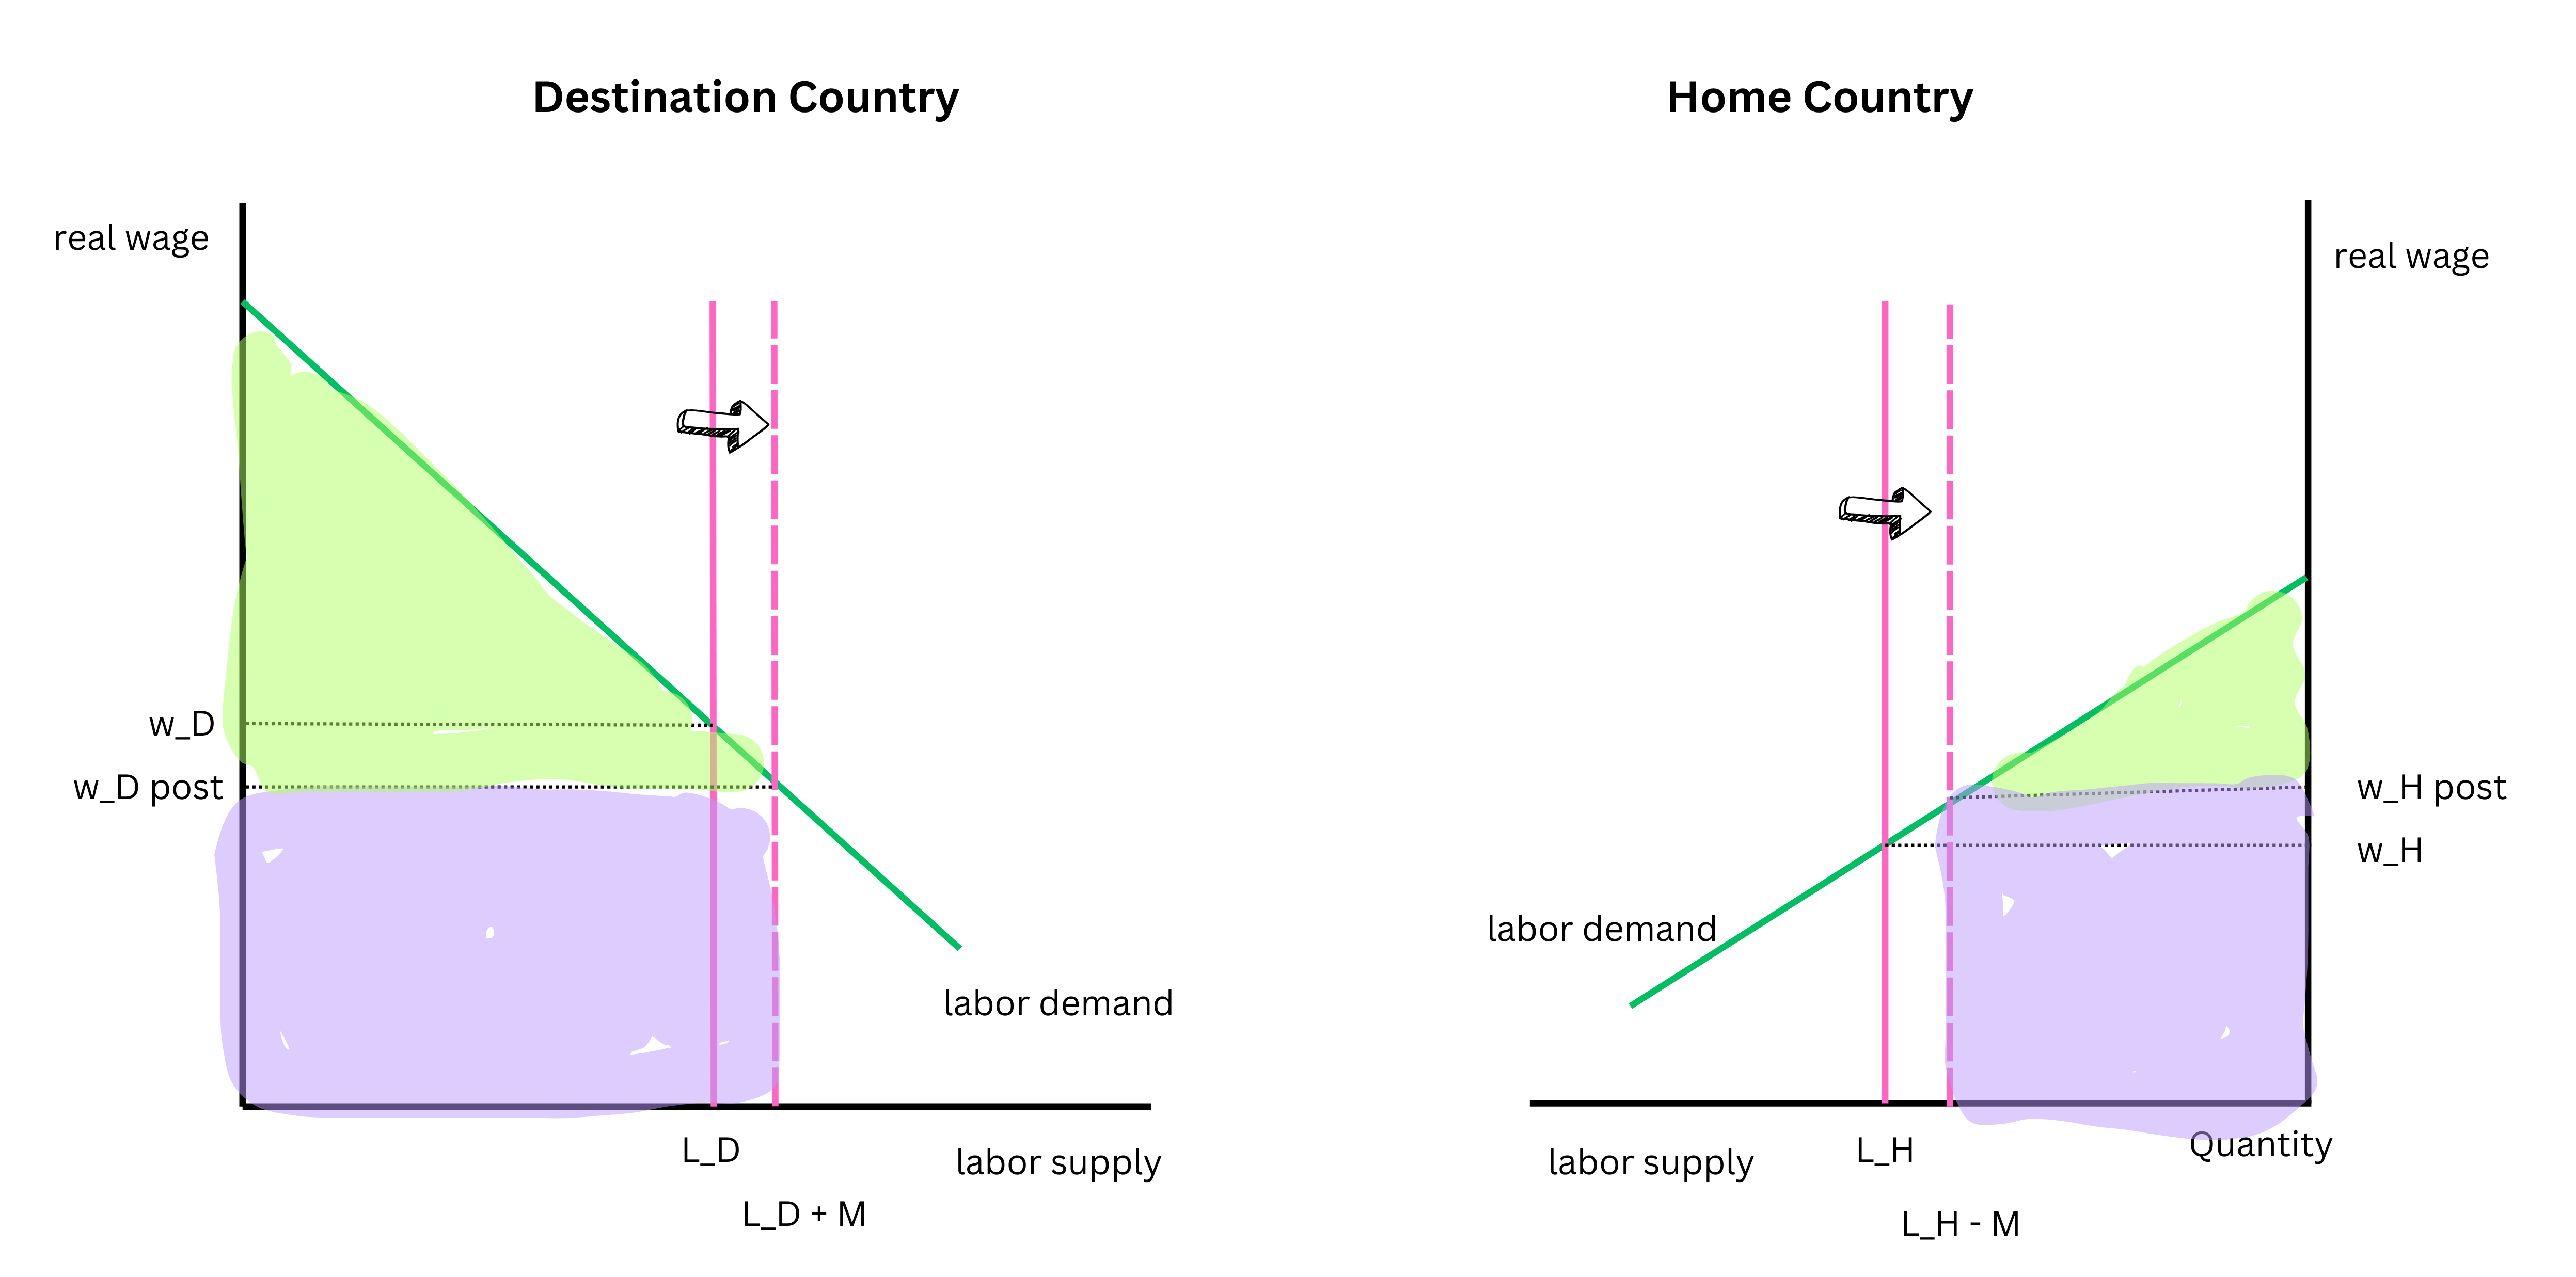
\includegraphics[width=\linewidth]{wages equlization through migration.png}
    \label{fig:enter-label}
\end{figure} 
\end{frame}

\begin{frame}{Graphic Illustration III}
\small
\textbf{Assumption:} A number of people ($M$) migrates from \textit{Home Country} to \textit{Destination Country}. They immediately contribute to the labor supply. We have free movement of people.
\begin{figure}
    \centering
    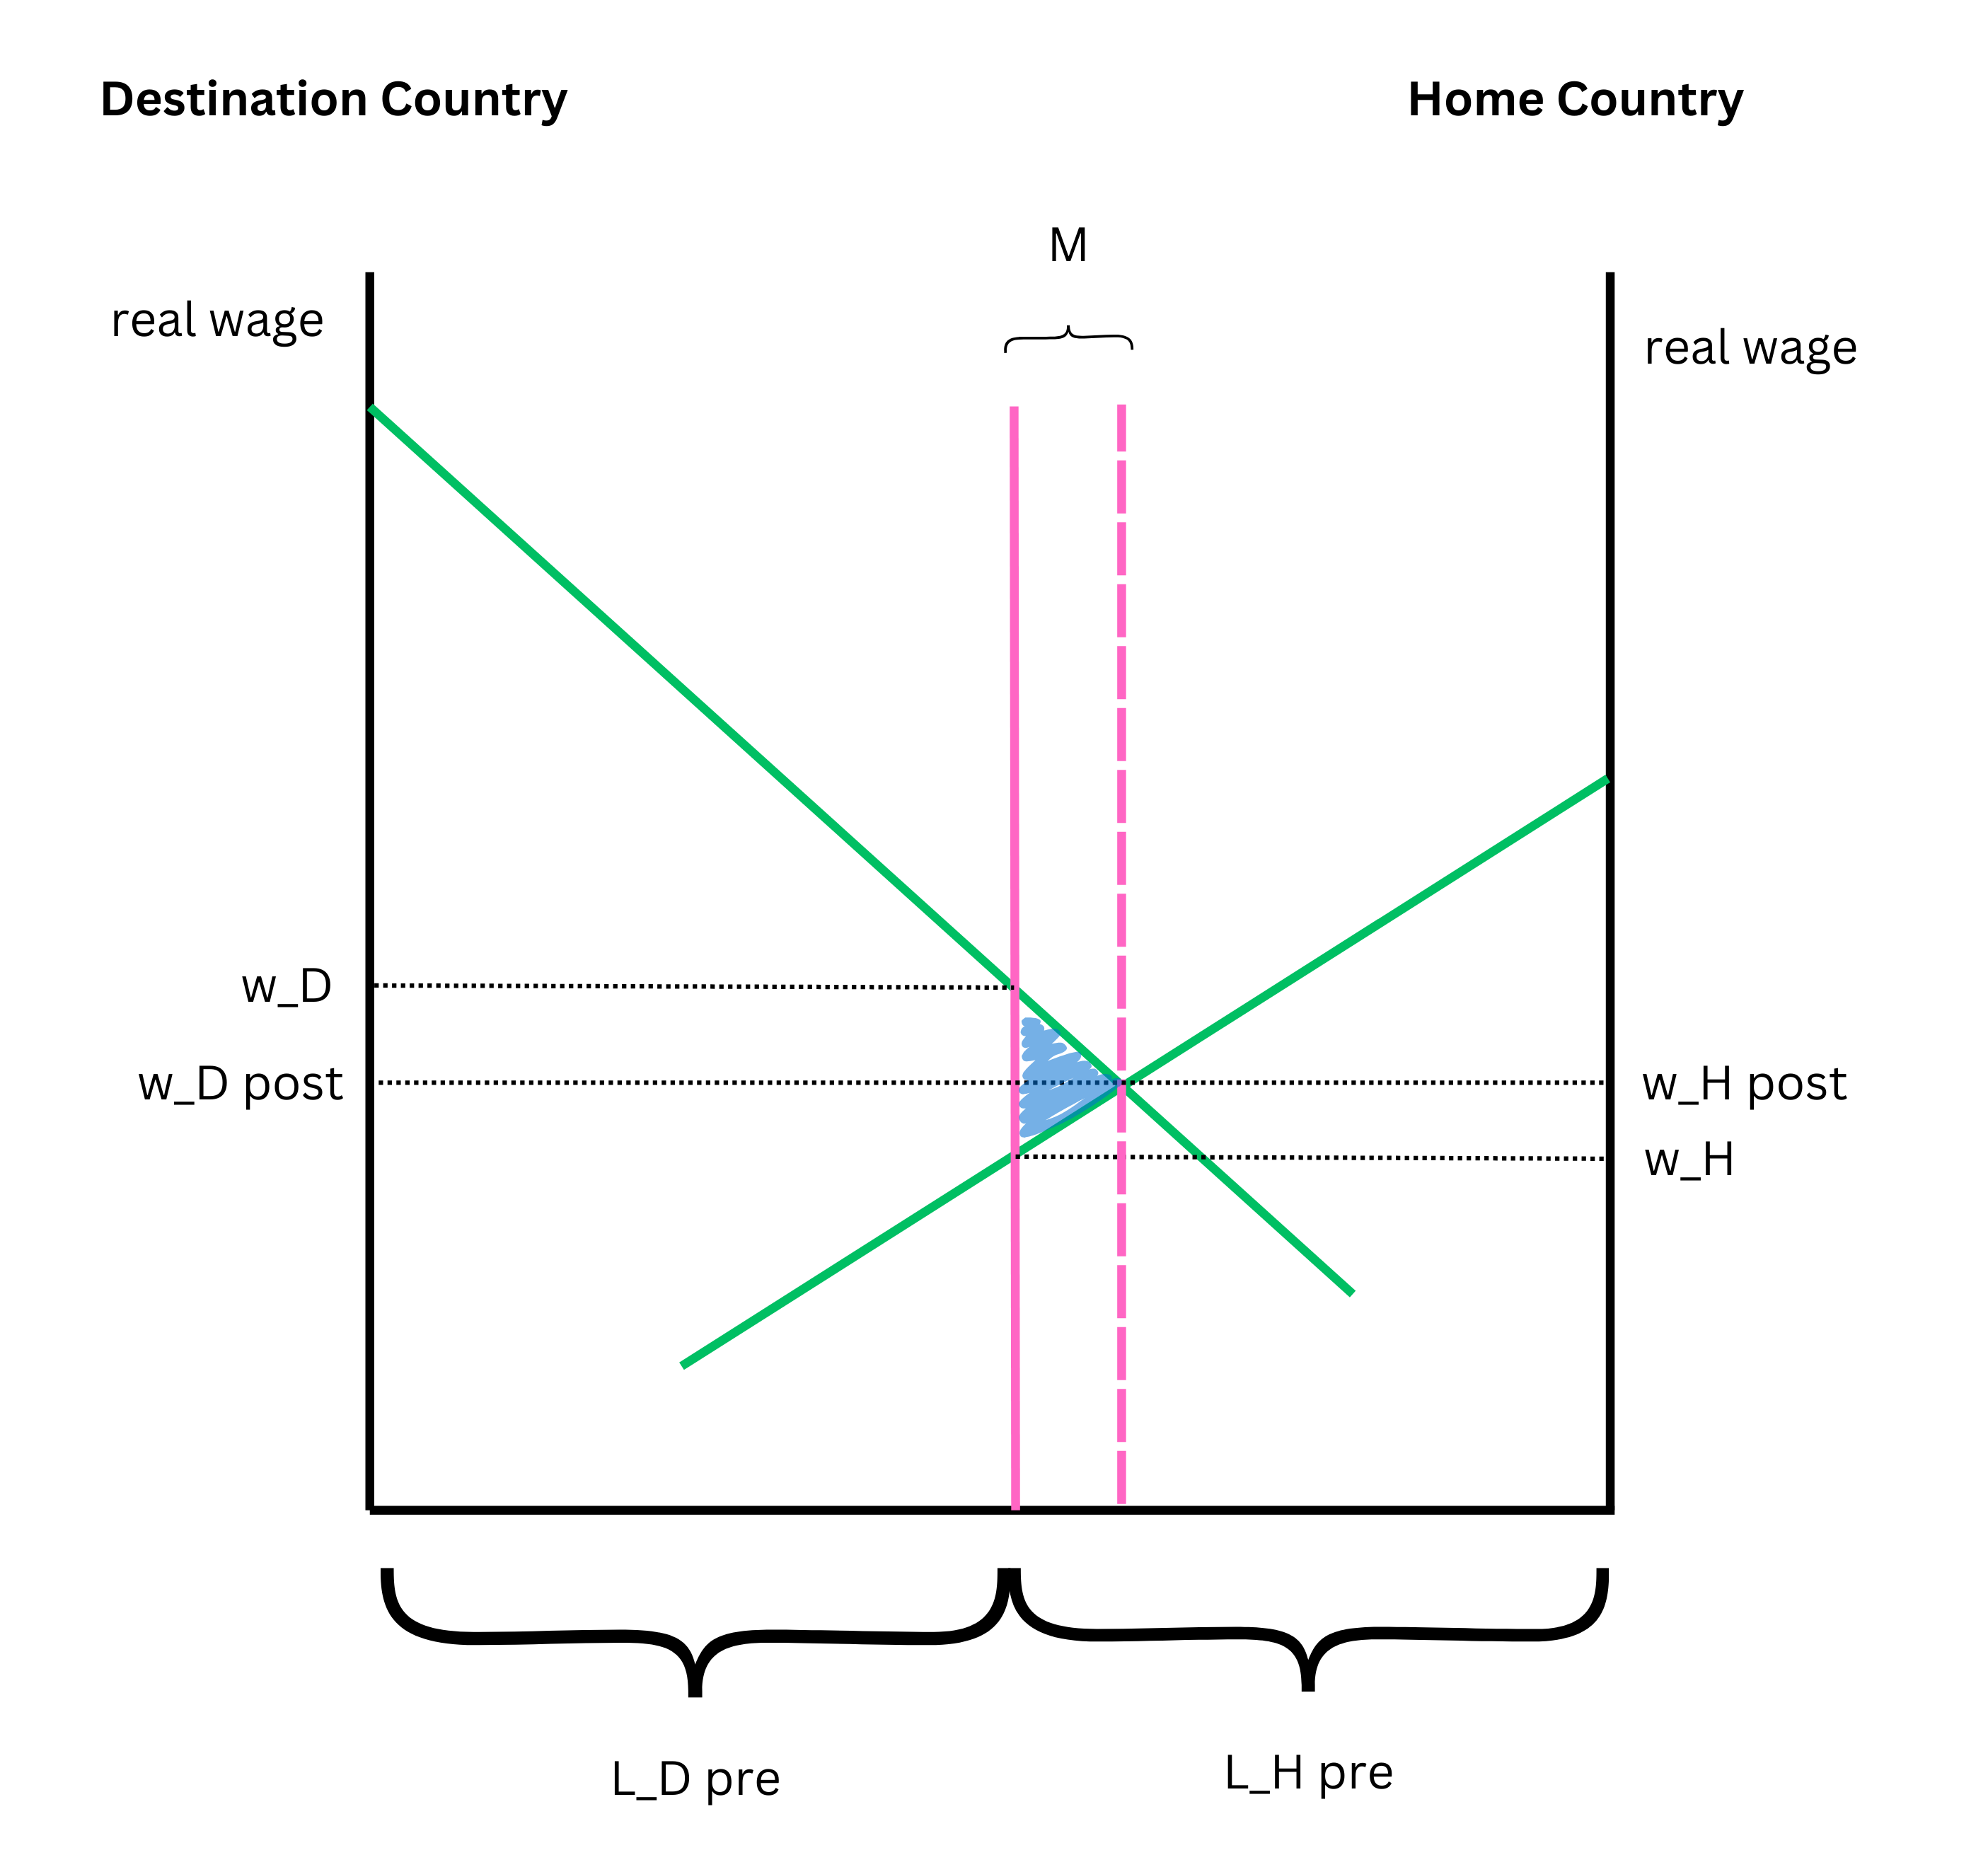
\includegraphics[width=0.6\linewidth]{wage equalization with free movement.png}
    \label{fig:enter-label}
\end{figure} 
\textbf{Finding: A free movement of people is expected to increase global welfare.}
\end{frame}

\begin{frame}{Actual Direction of Migration between 2015-2020}
    \begin{figure}
        \centering
        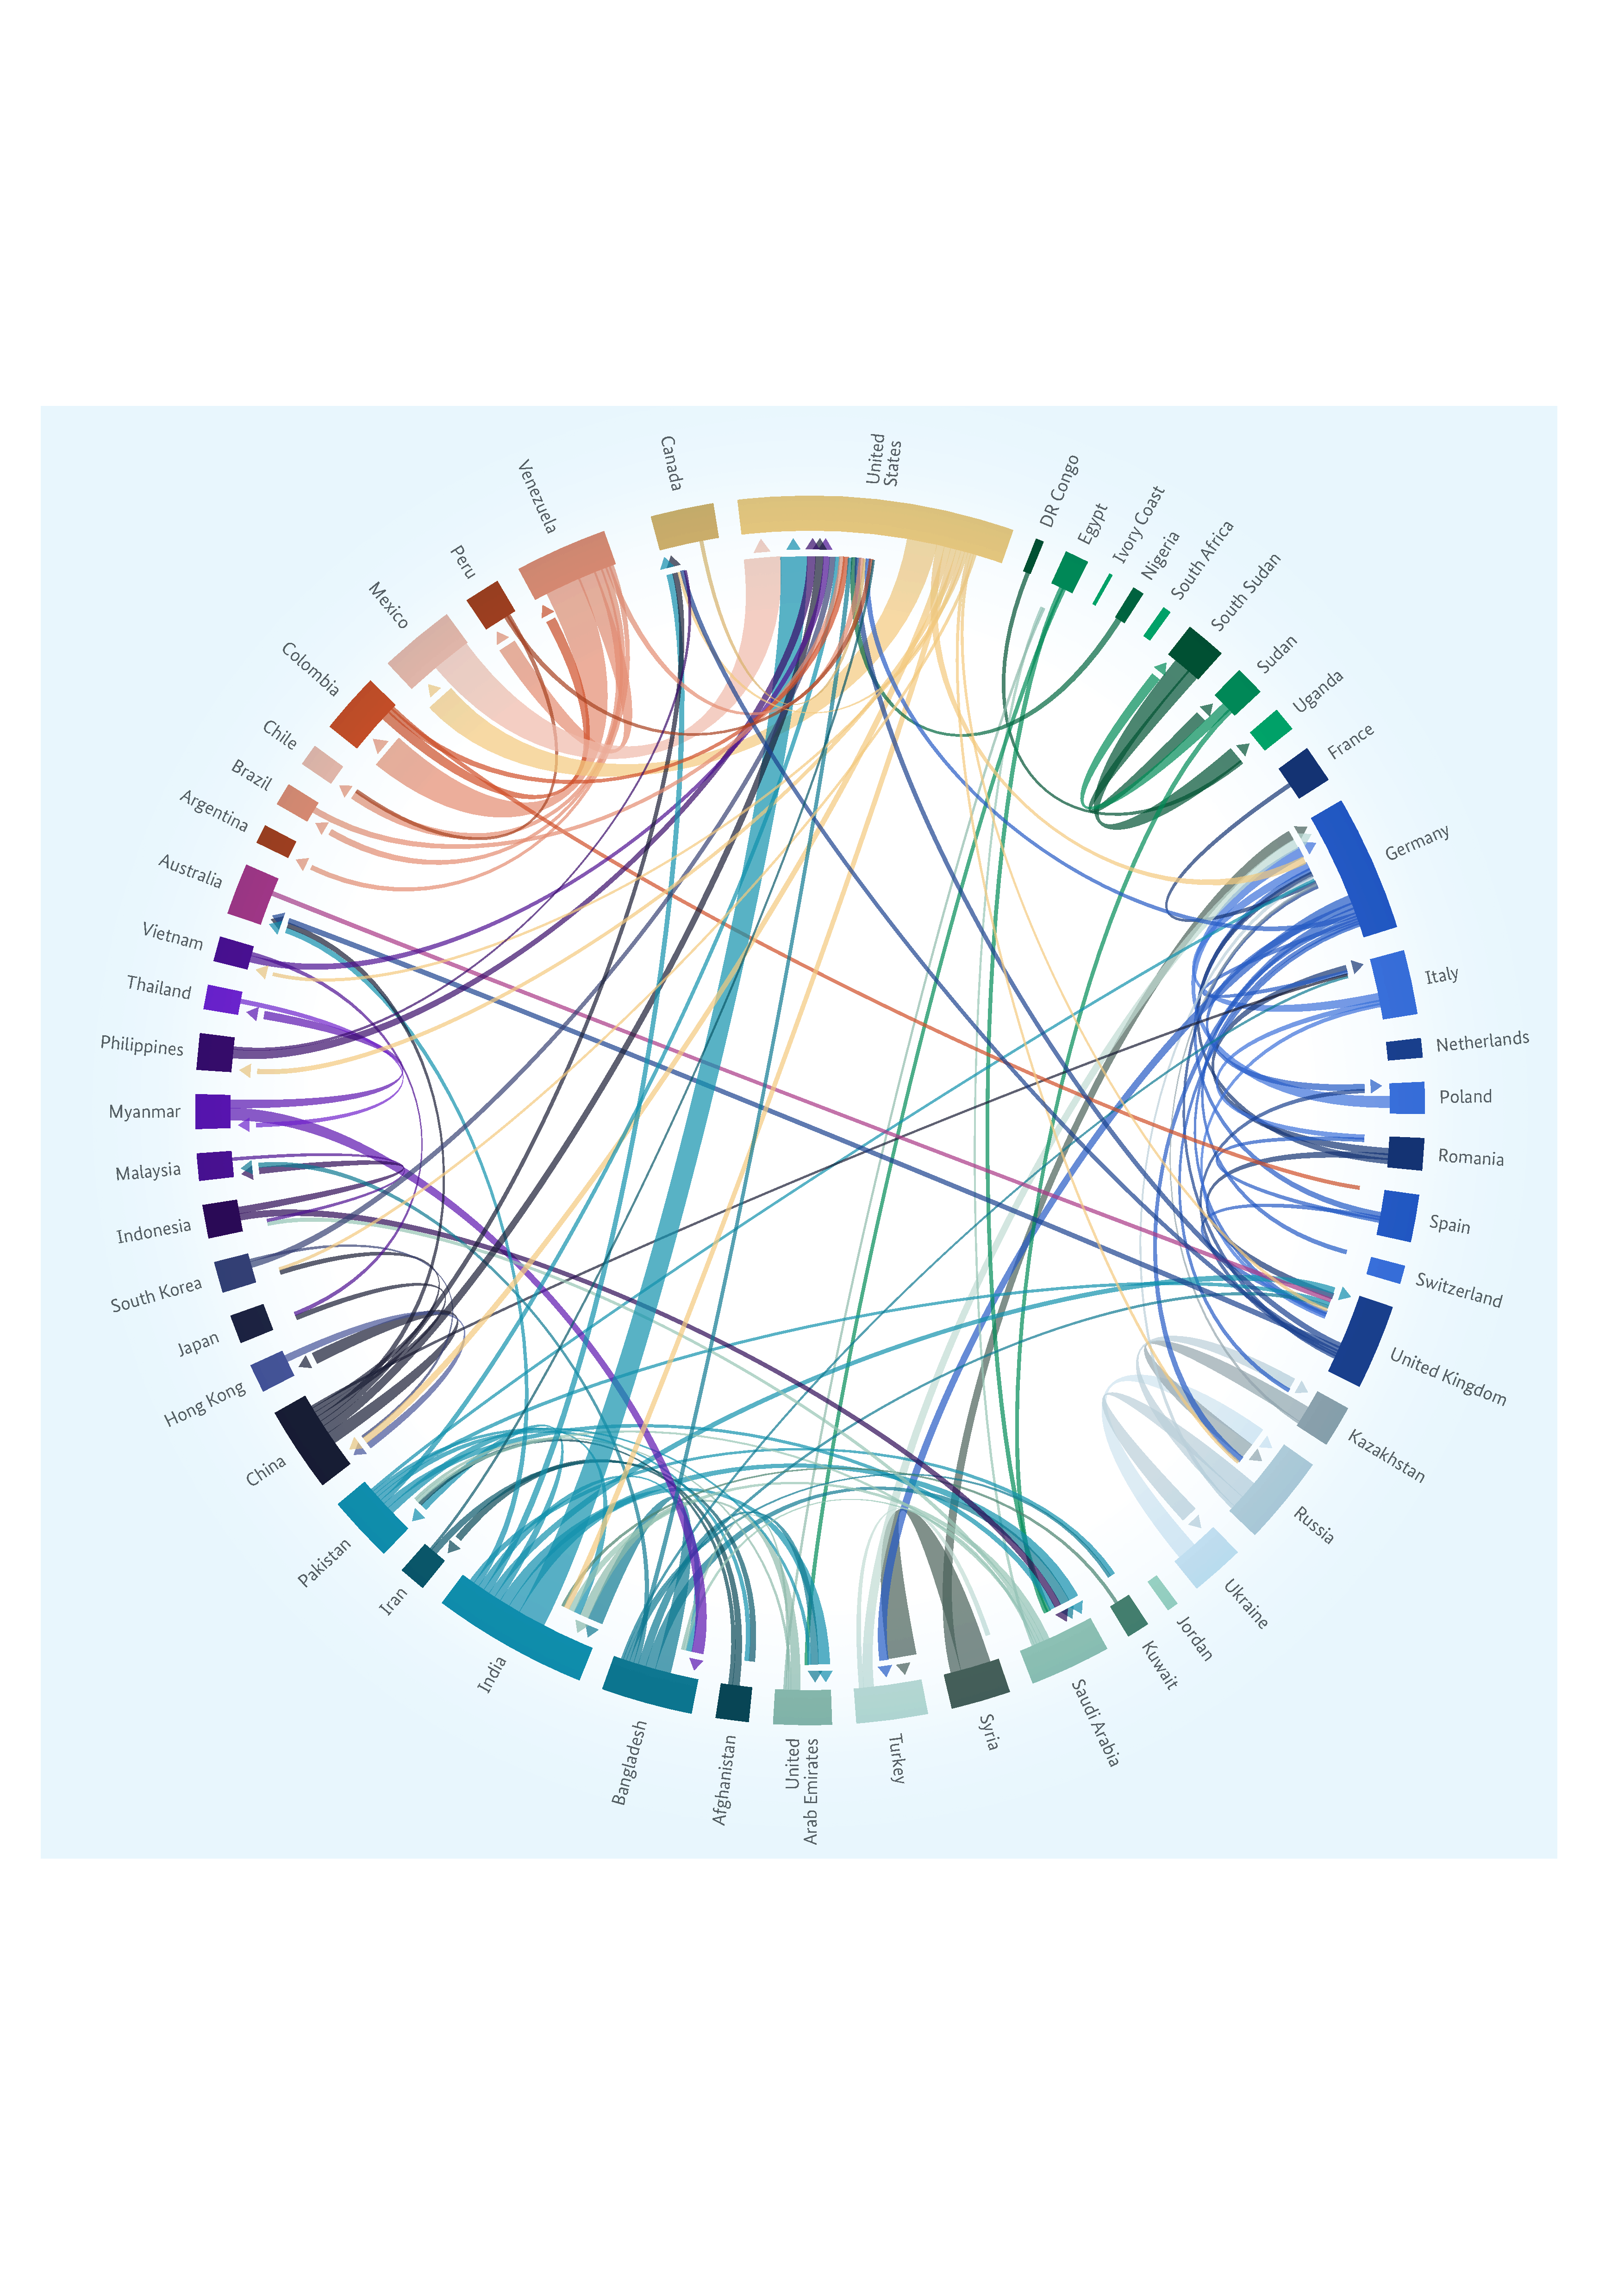
\includegraphics[width=0.7\linewidth]{migration flows.pdf}
        \label{fig:enter-label}
    \end{figure}
\end{frame}

\section{Political Drivers}

\begin{frame}{Civil Conflict, War}
    \textbf{Syrian Civil War (2011 -2024)}
\begin{itemize} \small
    \item More than 13 million Syrians were displaced, as least 6.7 million of those left the country.
    \item Reasons to migrate: forceful displacement, fear of persecution, fear for one's life, and the collapse of the economy, which left people in poverty and hunger.
\end{itemize}
    \textbf{Rwandan Genocide (1994)}
    \begin{itemize} \small
    \item Decades of internal conflicts between Hutu and Tutsi that were related to jurisdictional and economic inequality escalated.
    \item The civil war and genocide that occurred between April and July 1994 killed an estimated of 800,000 people. 
        \item Approximately 1 million Rwandans were internally displaced and 1.2 to 1.5 million fled to neighboring countries.
    \end{itemize}
\end{frame}

\begin{frame}{Political Persecution}
    \textbf{Jewish Migration in the first half of the 20th century}
    \begin{itemize} \small
        \item Millions of Jews fled Nazi Germany and occupied territories to escape systematic persecution, and deportation.
        \item Évian conference in 1938: of the 32 countries present, only the Dominican Republic agreed to relax racial quotas and accept more Jewish immigrants seeking to leave Germany.
    \end{itemize}
    \textbf{Huguenot Exodus from France (1685)}
    \begin{itemize} \small
        \item French Protestants (Huguenots) faced persecution and finally had their rights revoked in 1685. 
        \item Many fled to "protestant-friendly" countries such as England, the Netherlands, and Prussia.
        \item In the 16th century, Protestants made up around 10\% of the French population. In the 20th century, that share was down to around 1\%. 
    \end{itemize}
\end{frame}

\section{Social and Cultural Drivers}

\begin{frame}{Social Networks}
\textbf{Network effects}
    \begin{itemize} \small
        \item Social networks with earlier migrants from the same country facilitate the exchange of information and are thought to lower the costs of migrating.
        \item The migration of Irish people to the U.S. following the potato famine established Irish communities in cities like Boston, New York, and Chicago and providing connections, housing, and job opportunities.
        \item The same mechanism created chain migration for Italians and Mexicans migrating to the U.S., or Turks migrating to Germany.
    \end{itemize}
\end{frame}

\begin{frame}{Common Culture I}
    \begin{itemize} \small
        \item A “widely-spoken” native language in the destination country can be a pull-factor in international migration.
        \item Migration rates increase with linguistic proximity to the native language (\cite{migration_linguistic_proximity}).
        \item A shared colonial history that enforced a similar culture as well as language is still found to have a positive effect on migration patterns. Example: migration from former British India to the UK or from Algeria to France.
    \end{itemize}
\end{frame}

\begin{frame}{Common Culture II}
    \begin{itemize} \small
        \item  \textcite{dyen1992indoeuropean} show that cultural barriers and similarities explain patterns of migration flows better than traditional economic variables (pull and push factors) in a sample limited to developed countries.
        \item Cultural similarity is hard to measure quantitatively but there is a positive correlation between migration patterns and food and beverage preferences (\cite{food_preferences_and_migration}).
    \end{itemize}
\end{frame}

\section{Environmental Drivers}

\begin{frame}{Climate Change}
    \begin{itemize} \small
    \item Climate migration is a subset of environmental-related mobility that refers to movement driven by the impact of sudden or gradual climate-exacerbated disasters.
        \item The majority of people fleeing environmental disasters migrate over short distances (internally), and often temporarily. 
        \item Gradual shifts in the environment tend to impact more people than sudden disasters because they are less localized.
        \item Migration is thought to be the most direct human adaptation strategy to climate change.
    \end{itemize}
\end{frame}

\begin{frame}{Agricultural Productivity}
 % Set the width of the first column
 \small
Agricultural production is particularly vulnerable to climate change: altered temperature, precipitation, wind speed, crop growth cycles, the frequency of extreme weather events, and the occurrence of pests and diseases. \vspace{0.15cm}\\
    \textbf{Case Study: The Dust Bowl (1930s)}
    \begin{columns} % Start columns environment
    \column{0.6\textwidth}
    \begin{itemize} \small
        \item Drought in the Great Plains of the U.S.
        \item Internal migration: Between 1930 and 1940, about 3.5 million people moved out of the affected states. 
          \item Affected farmers specifically since crops could not grow, but nearly a third of all migrants were white-collar workers.
    \end{itemize}
    
    \column{0.4\textwidth} % Set the width of the second column
    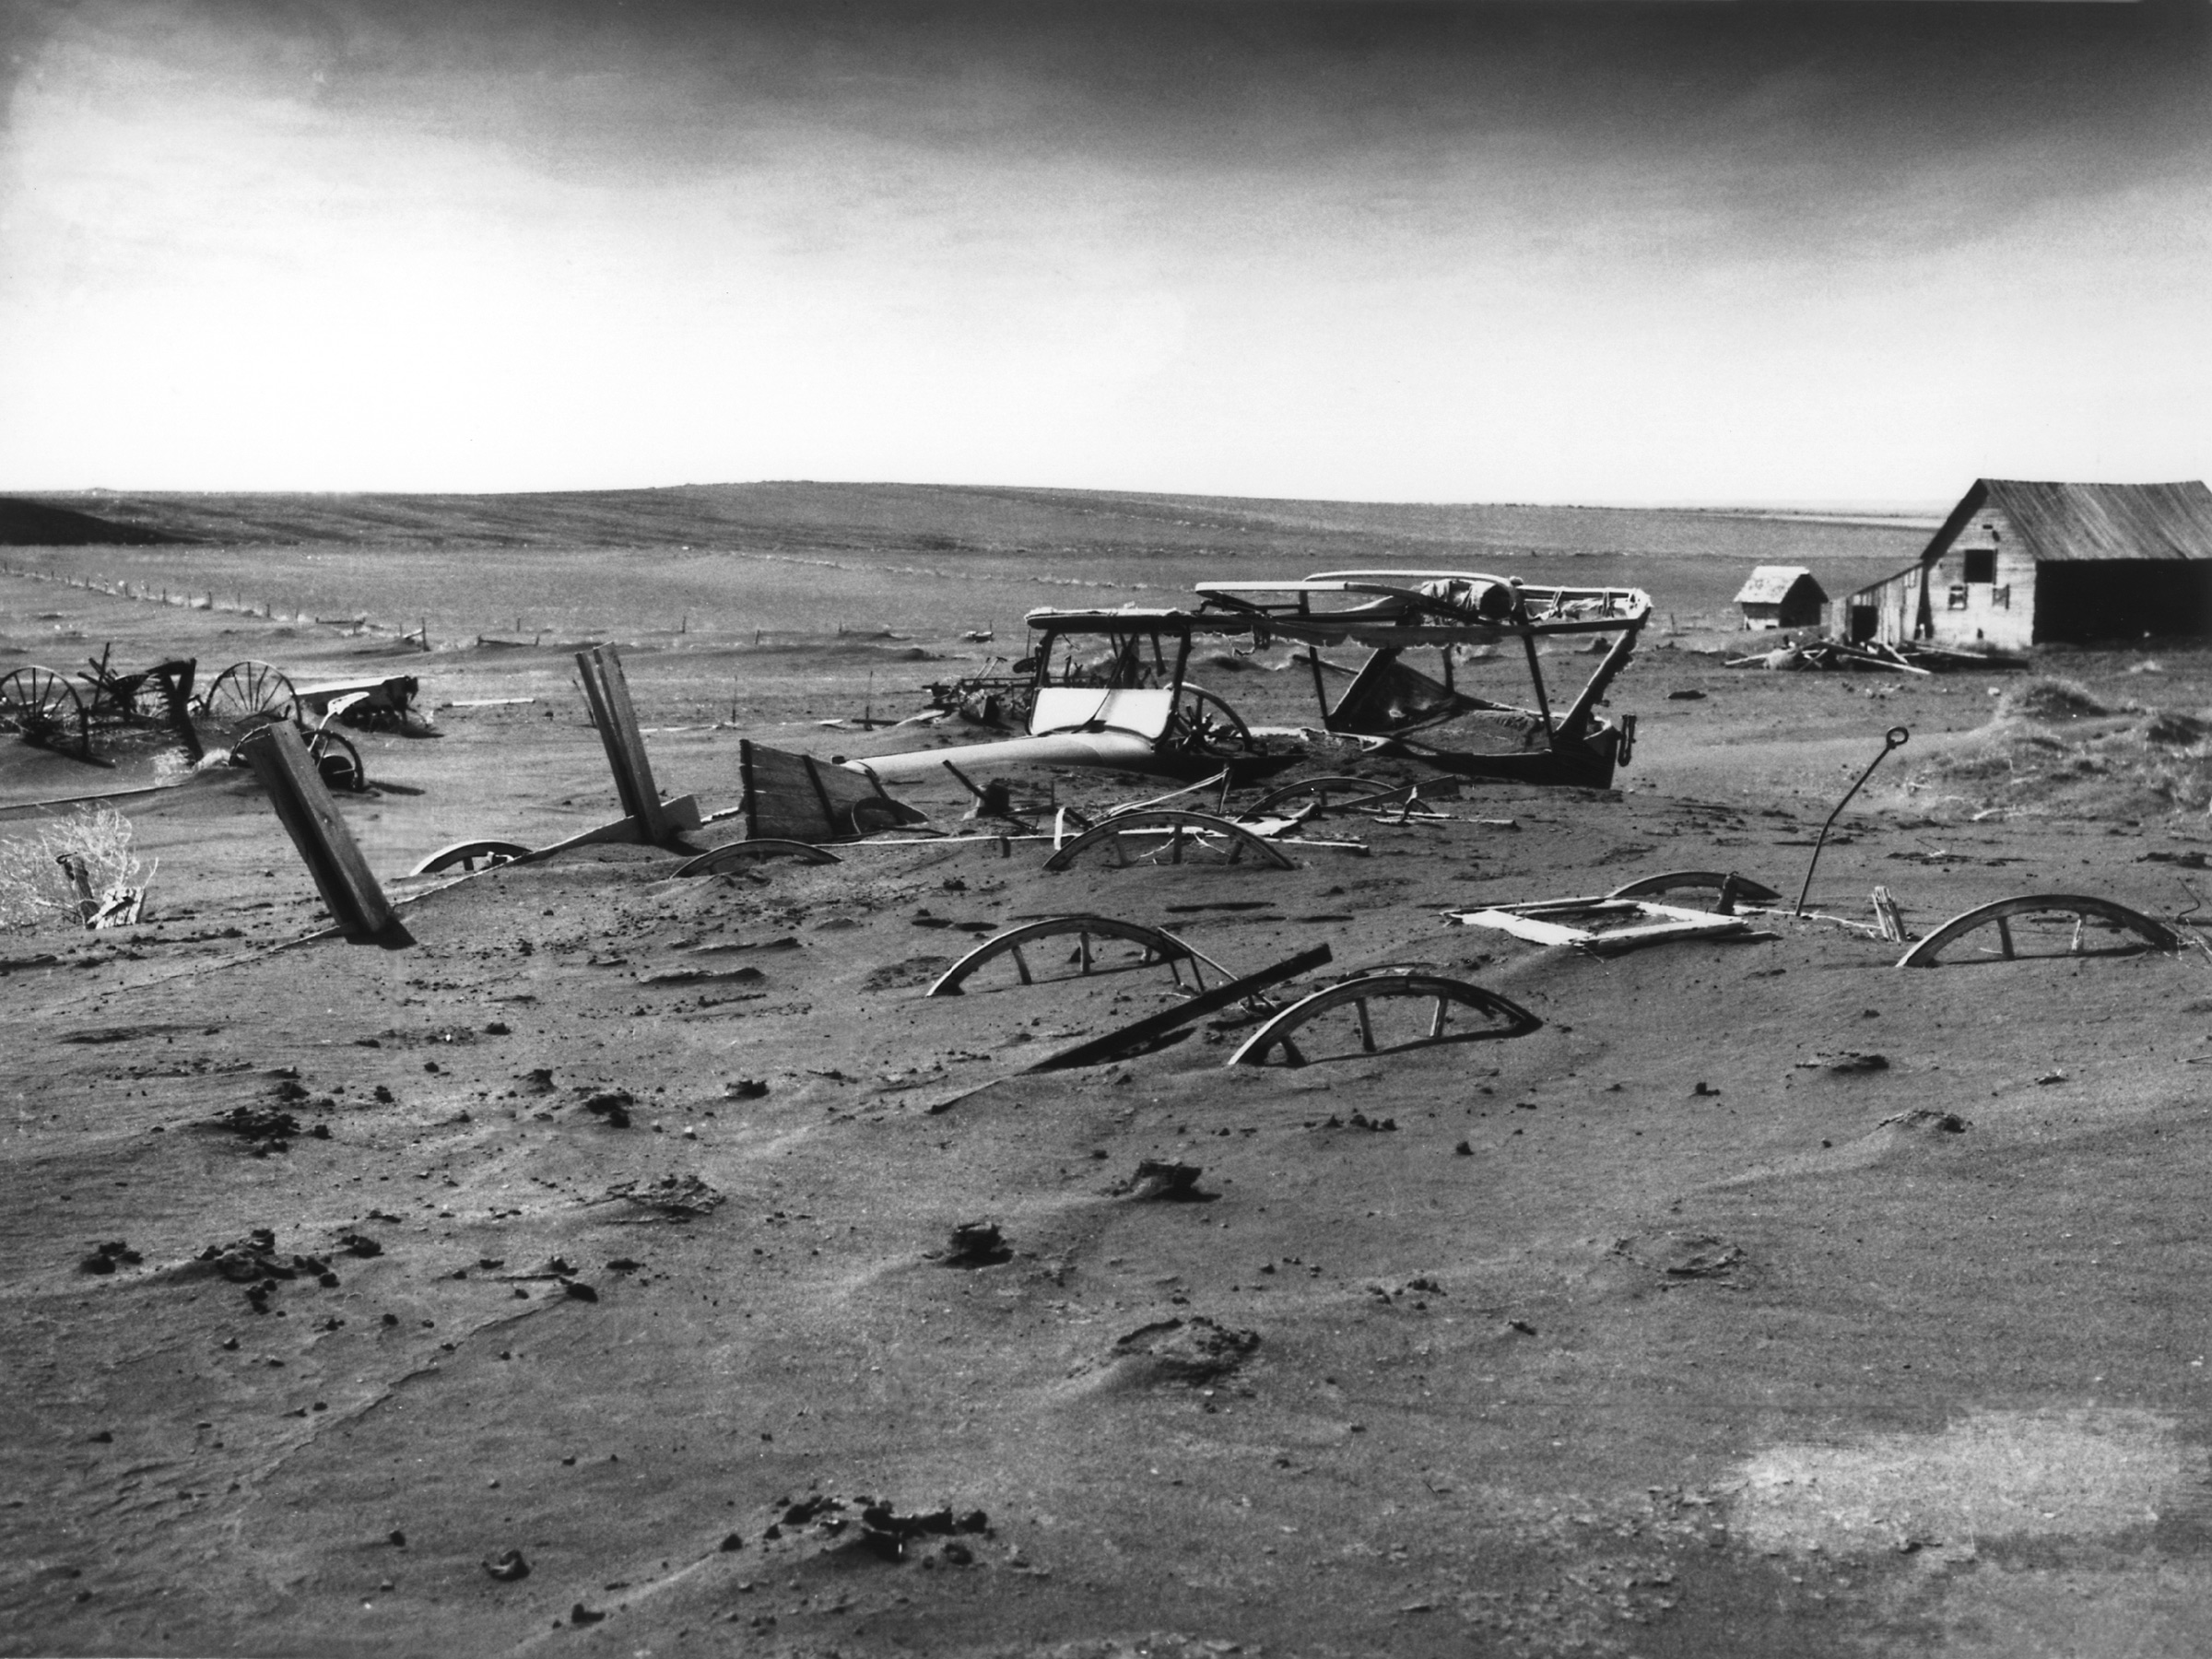
\includegraphics[width=\textwidth]{Dust_Bowl_-_Dallas,_South_Dakota_1936.png} % Replace with your image path
\end{columns}
\end{frame}

\begin{frame}{Climate-Induced Migration by 2050}
\begin{figure}
    \centering
    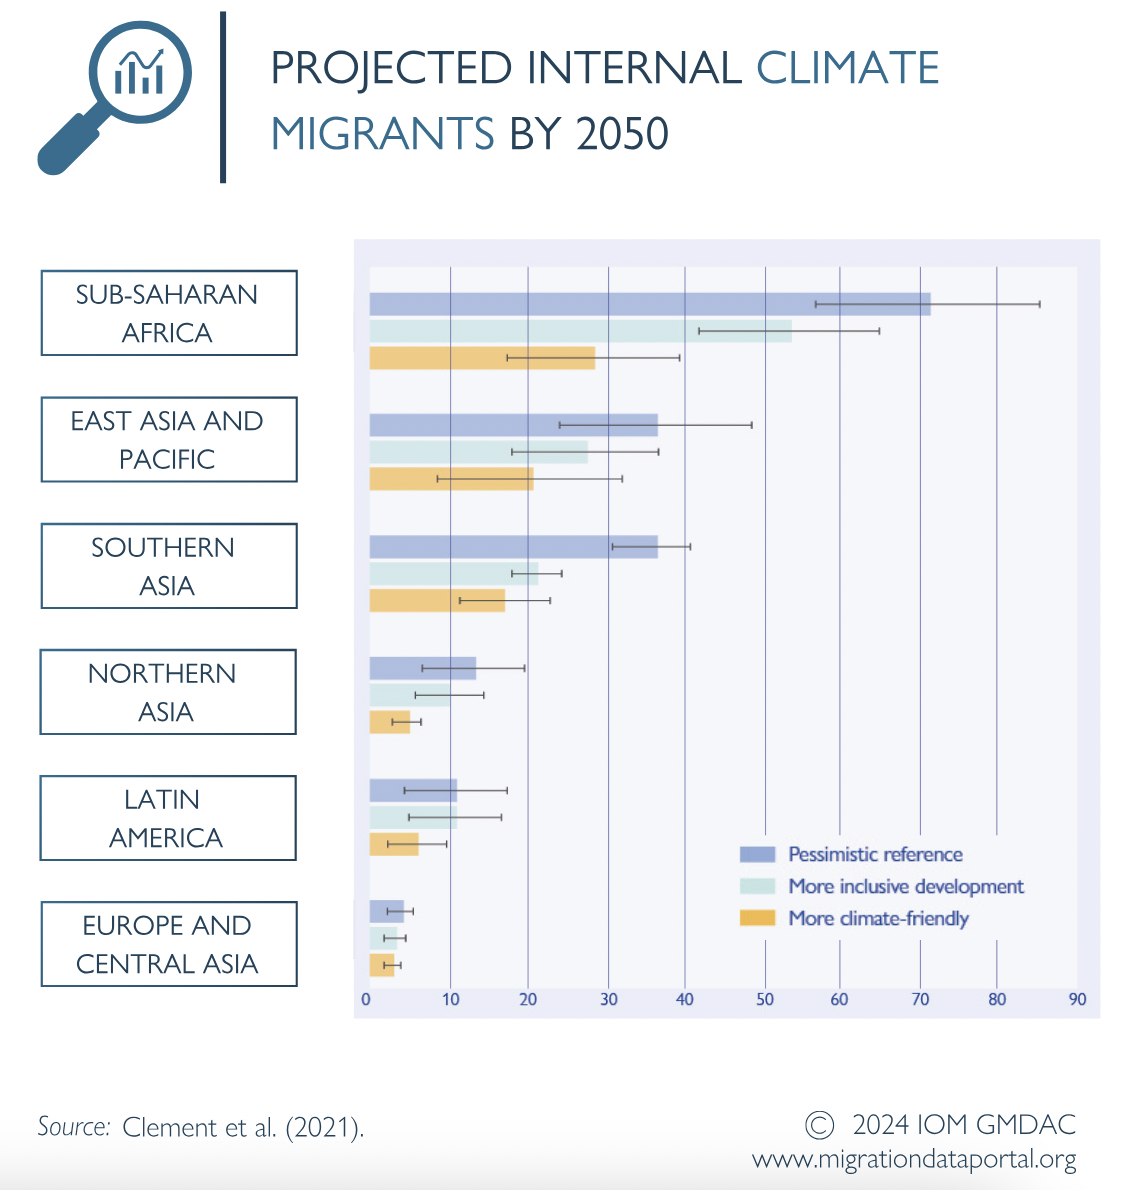
\includegraphics[width=0.6\linewidth]{projected migration.png}
    \label{fig:enter-label}
\end{figure}
\end{frame}

\begin{frame}{Take-Aways}
\begin{tcolorbox}
    \textbf{Take-Aways:}
    \begin{itemize} \small
        \item Geographical distance and average earnings differentials are used in economic models to explain the variation in migration patterns/flows.
        \item Distances in culture can act as a barrier to migration, while migrant communities and existing social networks act as a facilitating factor.
        \item Climate-induced migration is expected to be a major part of the migration we will see in the future.
        \item Focussing on economic differences in standards of living is not enough to understand people's motivation to migrate.
        \item The differentiation between voluntary migrants and forced migrants is not always clear.
    \end{itemize}
\end{tcolorbox}    
\end{frame}


\begin{frame}[allowframebreaks]{References}
    \printbibliography
\end{frame}


\end{document}

